% !TEX root = task-4-2-1.tex
% Editable task bank. Append new BankTask blocks at the end of the document.
\documentclass[12pt,a4paper]{article}
\usepackage{physics-textbook}
\usepackage{graphicx,needspace}
\usetikzlibrary{decorations.pathmorphing}
\newif\ifShowSolutions
\ifdefined\TutorEdition
  \ShowSolutionstrue
\else
  \ShowSolutionsfalse % Change to \ShowSolutionstrue to display solutions.
\fi
\newcounter{banktask}
\newsavebox{\BankTaskBox}
\newcommand{\BankTaskContent}[3]{%
  \noindent\textbf{\thebanktask.}\quad #2\par
  \ifShowSolutions
    \Needspace{50mm}% Keep the solution heading with its opening text or diagram.
    #3\par
    \ifdefined\TutorEdition
      \ifcsname TutorSource#1\endcsname
        \nopagebreak\smallskip{\small\csname TutorSource#1\endcsname\par}%
      \fi
    \fi
  \fi
}
\newcommand{\BankTask}[3]{%
  \refstepcounter{banktask}\par\medskip
  \sbox{\BankTaskBox}{\begin{minipage}{\linewidth}%
    \BankTaskContent{#1}{#2}{#3}\end{minipage}}%
  \ifdim\dimexpr\ht\BankTaskBox+\dp\BankTaskBox\relax>\dimexpr\textheight-20mm\relax
    \Needspace{35mm}\BankTaskContent{#1}{#2}{#3}%
  \else
    \Needspace{\dimexpr\ht\BankTaskBox+\dp\BankTaskBox\relax}%
    \noindent\usebox{\BankTaskBox}\par
  \fi
  \medskip
}
\begin{document}
\BookSubsection{4.2.1}{Закон отражения}


% Source 1732F3: https://ege.fipi.ru/bank/questions.php?search=1&proj=BA1F39653304A5B041B656915DC36B38&qid=1732F3
\BankTask{1732F3}{
Луч света падает на плоское зеркало. Угол отражения равен \(30^\circ\). Определите угол между падающим и отражённым лучами.
}{
\smallskip\noindent\textbf{Решение от GPT}\par
По закону отражения угол падения равен углу отражения: \(\alpha=\beta=30^\circ\). Угол между лучами \(\varphi=\alpha+\beta=60^\circ\).
Ответ: \(60^\circ\).
}

% Source 4D7B06: https://ege.fipi.ru/bank/questions.php?search=1&proj=BA1F39653304A5B041B656915DC36B38&qid=4D7B06
\BankTask{4D7B06}{
Луч света падает на плоское зеркало. Угол между падающим и отражённым лучами равен \(30^\circ\). Чему равен угол между падающим лучом и зеркалом?
}{
\smallskip\noindent\textbf{Решение от GPT}\par
Углы падения и отражения равны, поэтому угол падения \(\alpha=30^\circ/2=15^\circ\). Угол между падающим лучом и зеркалом равен \(90^\circ-\alpha=75^\circ\).
Ответ: \(75^\circ\).
}

% Source 29157: https://phys-ege.sdamgia.ru/problem?id=29157
\BankTask{29157}{
\begin{center}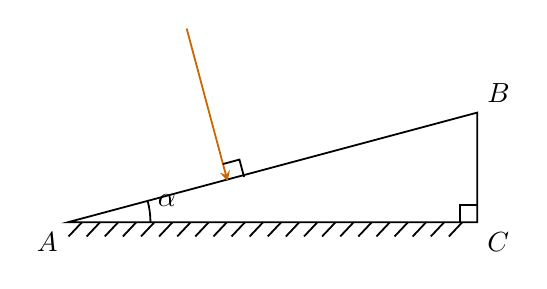
\begin{tikzpicture}[>=stealth,line width=.65pt]\draw (0,0)--(5.2,0)--(5.2,1.393)--cycle;\draw (1.05,0)arc(0:15:1.05)node[right]{$\alpha$};\foreach \x in {.18,.41,...,5.2}{\draw(\x,0)--++(-.17,-.18);}\draw (4.98,0)--(4.98,.22)--(5.2,.22);\draw[->,orange!80!black] (1.51,2.46)--(2.03,.52);\draw (1.971,.74)--(2.18,.796)--(2.239,.576);\node[below left]at(0,0){$A$};\node[above right]at(5.2,1.393){$B$};\node[below right]at(5.2,0){$C$};\end{tikzpicture}\end{center}

Нижняя грань AC прозрачного клина посеребрена и представляет собой плоское зеркало. Угол при вершине клина $\alpha = 15\ensuremath{{}^{\circ}}.$ Луч света падает из воздуха на клин перпендикулярно грани AB, преломляется и выходит в воздух через ту же грань AB, но уже под углом преломления $\beta = 60\ensuremath{{}^{\circ}}.$ Определите показатель преломления клина. Сделайте рисунок, поясняющий ход луча в клине.
}{
\smallskip\noindent\textbf{Решение}\par
\begin{center}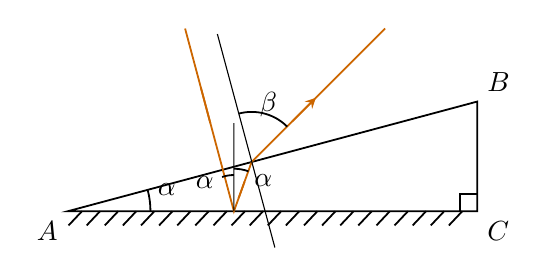
\begin{tikzpicture}[>=stealth,line width=.65pt]\draw (0,0)--(5.2,0)--(5.2,1.393)--cycle;\draw (1.05,0)arc(0:15:1.05)node[right]{$\alpha$};\foreach \x in {.18,.41,...,5.2}{\draw(\x,0)--++(-.17,-.18);}\draw (4.98,0)--(4.98,.22)--(5.2,.22);\draw[orange!80!black] (1.49,2.32)--(2.11,0)--(2.335,.626)--(4.03,2.32);\draw[->,orange!80!black](1.69,1.57)--(1.81,1.12) (2.17,.168)--(2.245,.375) (2.85,1.14)--(3.15,1.44);\draw[thin](2.11,0)--(2.11,1.12) (1.9,2.25)--(2.63,-.46);\draw (2.11,.46)arc(90:109:.46) (2.11,.54)arc(90:70:.54);\node[left]at(1.98,.37){$\alpha$};\node[right]at(2.24,.39){$\alpha$};\draw (2.17,1.24)arc(105:45:.638)node[above left]{$\beta$};\node[below left]at(0,0){$A$};\node[above right]at(5.2,1.393){$B$};\node[below right]at(5.2,0){$C$};\end{tikzpicture}\end{center}

$1$.  Луч, падающий на грань АВ, не преломляется, так как угол падения равен $0$\ensuremath{{}^{\circ}}. При падении на зеркальную грань $AC$ он падает под углом, который из геометрических соображений равен углу $\alpha .$ По закону отражения света угол отражения будет также равен $\alpha .$ 
$2$.  Данный луч падает на грань АВ под углом $\alpha _1=2 \alpha .$ По закону преломления света $\frac{\sin \alpha _1}{\sin \beta} = \frac{1}{n} ,$ откуда показатель преломления материала клина 

\[n= \frac{\sin \beta}{\sin 2 \alpha} = \frac{\sin 60 ^\circ}{\sin ( 2 \cdot 15 ^\circ )} = \sqrt{3} \approx 1{,}73.\]

Ответ: $1{,}73$.
}

\end{document}
